\section{Binomial distributed values}
This input is similar to the mixed input from the last subsection.
For this distribution the values are not chosen uniform random from one of the base distributions, but instead a value from every distribution is chosen and added together.
Hence the name overlapped distribution.
For this input the step limit was increased to $100\cdot n \ln n$.
The comparison with the step limit $10\cdot n \ln(n)$ is contained in the last subsubsection which compares the best variants.

\begin{figure}[h]
      \caption{Distribution of an overlapped input with \textasciitilde$U(1,999)$, \textasciitilde$B(1000,0.1)$, \textasciitilde$Geo(0.01)$, powerlaw dist with $\beta=-1.25$}
      \centering
      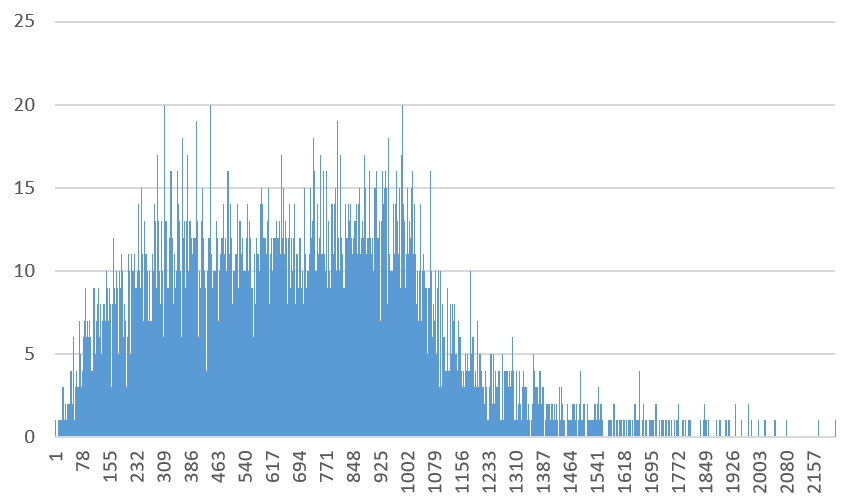
\includegraphics[width=0.7\textwidth]{figures/images/numberGenerator/overlapped.png}\label{fig:overlappedDistExample}
\end{figure}

Figure~\ref{fig:overlappedDistExample} looks completely different from figure~\ref{fig:mixedDistExample}.
No value is generated more than 20 times as opposed to the maximum amount of 350 for the mixed distribution.
In this figure no distribution is clearly visible.

The used distributions were \textasciitilde$U(1,49999)$, \textasciitilde$B(10000,0.1)$, \textasciitilde$Geo(0.001)$, powerlaw distribution with $\beta=-1.25$.
\subsection{RLS Comparison}
The following table lists the results for the RLS for inputs that are chosen from a powerlaw distribution with $\beta=-2.75$.


\makebox[\linewidth]{
\begin{tabular}{lp{3cm}p{6cm}p{6cm}}
\begin{tabular}[h]{cccccccc}
algo type&          RLS-N&   RLS-N&   RLS-R&   RLS-R&   RLS-R&   RLS-N&     RLS\\
algo param&           n=2&     n=4&     r=2&     r=4&     r=3&     n=3&       -\\
avg mut/change&     2.000&   4.000&   1.603&   2.553&   2.000&   2.728&   1.000\\
avg mut/step&       2.000&   4.000&   1.500&   2.500&   1.999&   3.000&   1.000\\
\hline
total avg count&      318&     434&     499&     579&     681& 518,428& 920,109\\
avg eval count&       318&     434&     499&     579&     681& 395,440&      50\\
max eval count&     1,648&   3,243&   3,094&   3,737&   4,717& 917,134&      50\\
min eval count&        20&      28&      11&      17&      16&       0&      50\\
\hline
fails&                  0&       0&       0&       0&       0&     234&     999\\
fail ratio&         0.000&   0.000&   0.000&   0.000&   0.000&   0.234&   0.999\\
avg fail dif&           -&       -&       -&       -&       -&       1&     254\\
\end{tabular}
\end{tabular}
}

For these inputs the variants of the RLS perform differently to the binomial input.
The only similarity is the RLS being the worst as the RLS is the only algorithm that did not find an optimal solution for every input.
If the RLS did find an optimal solution in those 5 cases it would instead be the best RLS variant.
The other algorithms are ranked by the probability of flipping only one bit.
This means at first the three RLS-R variants from 2 to 3 to 4 and then the same for the RLS-N variants.
So it does seem like moving mostly one element at once is better for the geometric input in comparison to two elements for the binomial distribution.
In the 5 cases where the RLS did not find an optimal solution it was most likely stuck in a local optimum.

\subsection{(1+1) EA Comparison}
The first table again shows the results for parameter $\beta=-2.75$

\makebox[\linewidth]{
\begin{tabular}{lp{3cm}p{6cm}p{6cm}}
\begin{tabular}[h]{ccccccccc}
algo type&          EA-SM&   EA-SM&   EA-SM&   EA-SM&      EA&   EA-SM&   EA-SM&   EA-SM\\
algo param&           3/n&     4/n&     2/n&     5/n&       -&    10/n&    50/n&   100/n\\
avg mut/change&     3.101&   3.968&   2.343&   4.859&   1.698&   9.732&  49.544&  99.494\\
avg mut/step&       2.999&   4.003&   2.002&   4.999&   1.001&   9.998&  49.998&  99.997\\
\hline
total avg count&      646&     701&     706&     857&   1,123&   1,508&   8,175&  15,485\\
avg eval count&       646&     701&     706&     857&   1,123&   1,508&   8,175&  15,485\\
max eval count&     5,346&   5,692&   3,415&   5,572&   7,001&  12,112&  52,831& 145,269\\
min eval count&        23&       4&      30&       9&      23&      14&      27&      69\\
\hline
fails&                  0&       0&       0&       0&       0&       0&       0&       0\\
fail ratio&         0.000&   0.000&   0.000&   0.000&   0.000&   0.000&   0.000&   0.000\\
avg fail dif&           -&       -&       -&       -&       -&       -&       -&       -\\
\end{tabular}
\end{tabular}
}

For the EA the result is also the inversion of the results for the OneMax equivalent.
The higher the mutation rate the better at least up to $n\le100$.
From mutation rate $p_m\le3/n$ the algorithm reaches the worst case at least once in 1000 runs.
If the algorithm did not manage to find an optimal solution the fitness was always the same.
So there was no run where any algorithm neither found a global nor the local optimum.
\subsection{pmut Comparison}
The first table again shows the results for parameter $\beta=-2.75$

\makebox[\linewidth]{
\scriptsize
\begin{tabular}{lp{3cm}p{6cm}p{6cm}}
\begin{tabular}[h]{cccccccccc}
algo type&           pmut&    pmut&    pmut&    pmut&    pmut&    pmut&    pmut&    pmut&    pmut\\
algo param&         -2.25&   -2.00&   -1.75&   -2.50&   -2.75&   -3.00&   -3.25&   -1.50&   -1.25\\
avg mut/change&     3.822&   6.266&  14.371&   2.804&   2.347&   1.995&   1.843&  38.318&  92.365\\
avg mut/step&       4.344&   8.504&  22.176&   2.878&   2.272&   1.933&   1.732&  70.476& 224.535\\
\hline
total avg count&      652&     668&     675&     688&     697&     718&     758&     785&   1,050\\
avg eval count&       652&     668&     675&     688&     697&     718&     758&     785&   1,050\\
max eval count&     4,340&   4,506&   5,616&   5,098&   9,140&   5,081&   6,189&   6,542&   7,837\\
min eval count&        14&       4&       9&      12&      27&      10&      11&      21&       7\\
\hline
fails&                  0&       0&       0&       0&       0&       0&       0&       0&       0\\
fail ratio&         0.000&   0.000&   0.000&   0.000&   0.000&   0.000&   0.000&   0.000&   0.000\\
avg fail dif&           -&       -&       -&       -&       -&       -&       -&       -&       -\\
\end{tabular}
\end{tabular}
}

The ideal value for $\beta$ seems to be around -1.75 as the runtime increases for the two neighbour values.
Even the worst value still manages find an optimal solution within double the time of the best value.
The importance of the parameter is therefore not as important as for other inputs.
\subsection{Comparison of the best variants}
The first table again shows the results for parameter $\beta=-2.75$

\makebox[\linewidth]{
\begin{tabular}{lp{3cm}p{6cm}p{6cm}}
\begin{tabular}[h]{cccc}
algo type&        RLS-N& EA-SM&  pmut\\
algo param&         n=2&   3/n& -2.25\\
avg mut/change&   2.000& 3.092& 3.965\\
avg mut/step&     2.000& 2.999& 4.339\\
\hline
total avg count&    302&   677&   691\\
avg eval count&     302&   677&   691\\
max eval count&   1,610& 6,404& 5,205\\
min eval count&       9&    33&    17\\
\hline
fails&                0&     0&     0\\
fail ratio&       0.000& 0.000& 0.000\\
avg fail dif&         -&     -&     -\\
\end{tabular}
\end{tabular}
}

The results for this experiment are as expected.
All three algorithms find the optimal value within the time limit.
The RLS performs better than the (1+1) EA because it does only single bit flips.
The $pmut_{-3.25}$ perform better than the standard (1+1) EA although flipping more bits on average.
This is most likely cause by the few steps where $pmut$ flips many bits which increase the average.
But $pmut$ most likely chooses to flip only one bit more often as the (1+1) EA.

TODO insert comparison with multiple values of n.
\section{Geometric distributed values}
This input is similar to the mixed input from the last subsection.
For this distribution the values are not chosen uniform random from one of the base distributions, but instead a value from every distribution is chosen and added together.
Hence the name overlapped distribution.
For this input the step limit was increased to $100\cdot n \ln n$.
The comparison with the step limit $10\cdot n \ln(n)$ is contained in the last subsubsection which compares the best variants.

\begin{figure}[h]
      \caption{Distribution of an overlapped input with \textasciitilde$U(1,999)$, \textasciitilde$B(1000,0.1)$, \textasciitilde$Geo(0.01)$, powerlaw dist with $\beta=-1.25$}
      \centering
      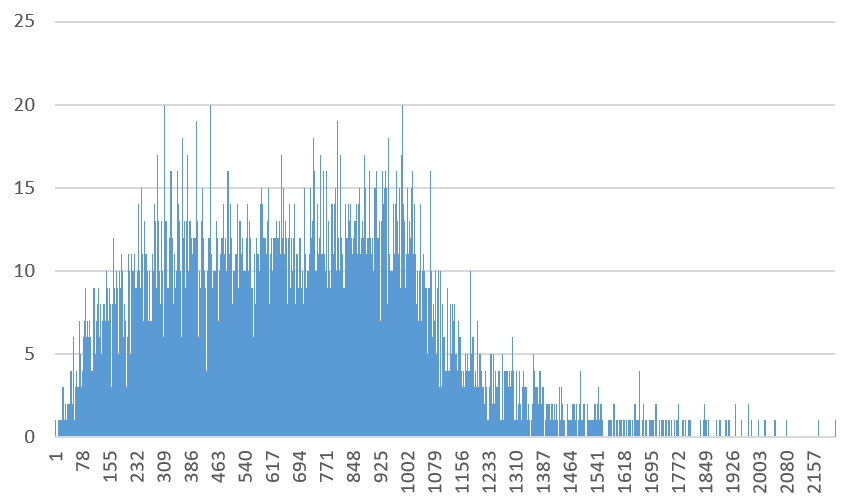
\includegraphics[width=0.7\textwidth]{figures/images/numberGenerator/overlapped.png}\label{fig:overlappedDistExample}
\end{figure}

Figure~\ref{fig:overlappedDistExample} looks completely different from figure~\ref{fig:mixedDistExample}.
No value is generated more than 20 times as opposed to the maximum amount of 350 for the mixed distribution.
In this figure no distribution is clearly visible.

The used distributions were \textasciitilde$U(1,49999)$, \textasciitilde$B(10000,0.1)$, \textasciitilde$Geo(0.001)$, powerlaw distribution with $\beta=-1.25$.
\subsection{RLS Comparison}
The following table lists the results for the RLS for inputs that are chosen from a powerlaw distribution with $\beta=-2.75$.


\makebox[\linewidth]{
\begin{tabular}{lp{3cm}p{6cm}p{6cm}}
\begin{tabular}[h]{cccccccc}
algo type&         RLS-R&  RLS-R&  RLS-R&  RLS-N&  RLS-N&  RLS-N&    RLS\\
algo param&          r=2&    r=3&    r=4&    n=2&    n=3&    n=4&      -\\
avg mut/change&    1.477&  1.959&  2.431&  2.000&  3.000&  4.000&  1.000\\
avg mut/step&      1.500&  2.001&  2.501&  2.000&  3.000&  4.000&  1.000\\
\hline
total avg count&   2,592&  2,945&  3,259&  3,497&  4,463&  5,345&  6,650\\
avg eval count&    2,592&  2,945&  3,259&  3,497&  4,463&  5,345&  2,055\\
max eval count&   19,845& 23,932& 28,532& 23,824& 30,881& 41,600& 25,889\\
min eval count&        8&     22&     19&     18&     43&     19&     23\\
\hline
fails&                 0&      0&      0&      0&      0&      0&      5\\
fail ratio&        0.000&  0.000&  0.000&  0.000&  0.000&  0.000&  0.005\\
avg fail dif&          -&      -&      -&      -&      -&      -&      1\\
\end{tabular}
\end{tabular}
}

For these inputs the variants of the RLS perform differently to the binomial input.
The only similarity is the RLS being the worst as the RLS is the only algorithm that did not find an optimal solution for every input.
If the RLS did find an optimal solution in those 5 cases it would instead be the best RLS variant.
The other algorithms are ranked by the probability of flipping only one bit.
This means at first the three RLS-R variants from 2 to 3 to 4 and then the same for the RLS-N variants.
So it does seem like moving mostly one element at once is better for the geometric input in comparison to two elements for the binomial distribution.
In the 5 cases where the RLS did not find an optimal solution it was most likely stuck in a local optimum.

\subsection{(1+1) EA Comparison}
The first table again shows the results for parameter $\beta=-2.75$

\makebox[\linewidth]{
\begin{tabular}{lp{3cm}p{6cm}p{6cm}}
\begin{tabular}[h]{ccccccccc}
algo type&          EA-SM&      EA&   EA-SM&   EA-SM&   EA-SM&   EA-SM&   EA-SM&   EA-SM\\
algo param&           2/n&       -&     3/n&     4/n&     5/n&    10/n&    50/n&   100/n\\
avg mut/change&     2.255&   1.554&   3.038&   3.948&   4.883&   9.821&  49.798&  99.814\\
avg mut/step&       2.000&   1.000&   3.000&   4.001&   5.000&   9.999&  49.998& 100.001\\
\hline
total avg count&    3,712&   3,833&   4,195&   4,472&   5,465&   8,282&  21,648&  29,404\\
avg eval count&     3,712&   3,833&   4,195&   4,472&   5,465&   8,282&  21,648&  29,404\\
max eval count&    39,593&  53,450&  33,598&  42,449&  55,717&  65,522& 149,048& 281,857\\
min eval count&        18&      13&      15&      14&      25&      23&      46&      17\\
\hline
fails&                  0&       0&       0&       0&       0&       0&       0&       0\\
fail ratio&         0.000&   0.000&   0.000&   0.000&   0.000&   0.000&   0.000&   0.000\\
avg fail dif&           -&       -&       -&       -&       -&       -&       -&       -\\
\end{tabular}
\end{tabular}
}

For the EA the result is also the inversion of the results for the OneMax equivalent.
The higher the mutation rate the better at least up to $n\le100$.
From mutation rate $p_m\le3/n$ the algorithm reaches the worst case at least once in 1000 runs.
If the algorithm did not manage to find an optimal solution the fitness was always the same.
So there was no run where any algorithm neither found a global nor the local optimum.
\subsection{pmut Comparison}
The first table again shows the results for parameter $\beta=-2.75$

\makebox[\linewidth]{
\scriptsize
\begin{tabular}{lp{3cm}p{6cm}p{6cm}}
\begin{tabular}[h]{cccccccccc}
algo type&           pmut&    pmut&    pmut&    pmut&    pmut&    pmut&    pmut&    pmut&    pmut\\
algo param&         -3.25&   -3.00&   -2.50&   -2.75&   -2.25&   -2.00&   -1.75&   -1.50&   -1.25\\
avg mut/change&     1.682&   1.872&   2.688&   2.150&   3.704&   6.938&  16.352&  41.906& 107.789\\
avg mut/step&       1.730&   1.936&   2.918&   2.267&   4.355&   8.463&  22.369&  70.989& 225.029\\
\hline
total avg count&    2,575&   2,732&   2,734&   2,776&   2,809&   3,165&   3,486&   4,389&   6,151\\
avg eval count&     2,575&   2,732&   2,734&   2,776&   2,809&   3,165&   3,486&   4,389&   6,151\\
max eval count&    73,911&  34,215&  75,791&  42,620&  25,352&  31,966&  37,725&  50,454&  55,022\\
min eval count&        33&      17&      11&       0&      35&       9&       5&      23&      19\\
\hline
fails&                  0&       0&       0&       0&       0&       0&       0&       0&       0\\
fail ratio&         0.000&   0.000&   0.000&   0.000&   0.000&   0.000&   0.000&   0.000&   0.000\\
avg fail dif&           -&       -&       -&       -&       -&       -&       -&       -&       -\\
\end{tabular}
\end{tabular}
}

The ideal value for $\beta$ seems to be around -1.75 as the runtime increases for the two neighbour values.
Even the worst value still manages find an optimal solution within double the time of the best value.
The importance of the parameter is therefore not as important as for other inputs.
\subsection{Comparison of the best variants}
The first table again shows the results for parameter $\beta=-2.75$

\makebox[\linewidth]{
\begin{tabular}{lp{3cm}p{6cm}p{6cm}}
\begin{tabular}[h]{cccc}
algo type&         RLS-R&   pmut&  EA-SM\\
algo param&          r=2&  -3.25&    2/n\\
avg mut/change&    1.483&  1.693&  2.258\\
avg mut/step&      1.500&  1.729&  2.001\\
\hline
total avg count&   2,407&  2,695&  3,421\\
avg eval count&    2,407&  2,695&  3,421\\
max eval count&   23,155& 57,661& 52,762\\
min eval count&       19&     11&     19\\
\hline
fails&                 0&      0&      0\\
fail ratio&        0.000&  0.000&  0.000\\
avg fail dif&          -&      -&      -\\
\end{tabular}
\end{tabular}
}

The results for this experiment are as expected.
All three algorithms find the optimal value within the time limit.
The RLS performs better than the (1+1) EA because it does only single bit flips.
The $pmut_{-3.25}$ perform better than the standard (1+1) EA although flipping more bits on average.
This is most likely cause by the few steps where $pmut$ flips many bits which increase the average.
But $pmut$ most likely chooses to flip only one bit more often as the (1+1) EA.

TODO insert comparison with multiple values of n.
\section{Uniform distributed inputs}
This input is similar to the mixed input from the last subsection.
For this distribution the values are not chosen uniform random from one of the base distributions, but instead a value from every distribution is chosen and added together.
Hence the name overlapped distribution.
For this input the step limit was increased to $100\cdot n \ln n$.
The comparison with the step limit $10\cdot n \ln(n)$ is contained in the last subsubsection which compares the best variants.

\begin{figure}[h]
      \caption{Distribution of an overlapped input with \textasciitilde$U(1,999)$, \textasciitilde$B(1000,0.1)$, \textasciitilde$Geo(0.01)$, powerlaw dist with $\beta=-1.25$}
      \centering
      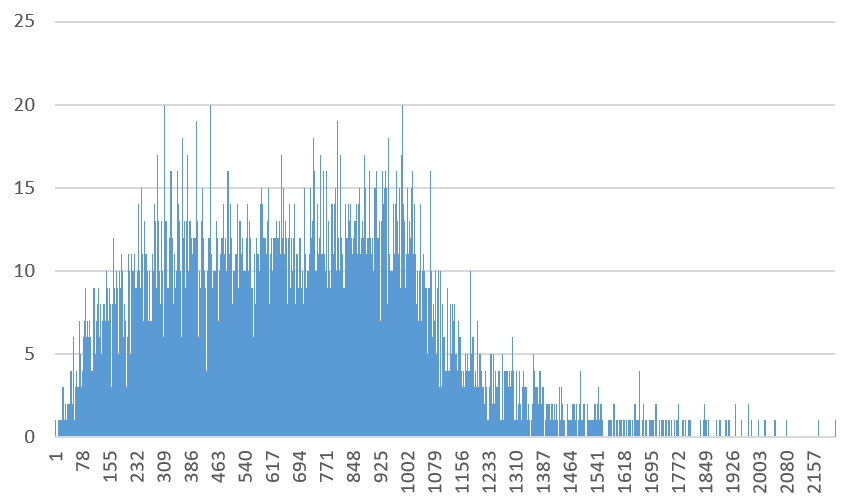
\includegraphics[width=0.7\textwidth]{figures/images/numberGenerator/overlapped.png}\label{fig:overlappedDistExample}
\end{figure}

Figure~\ref{fig:overlappedDistExample} looks completely different from figure~\ref{fig:mixedDistExample}.
No value is generated more than 20 times as opposed to the maximum amount of 350 for the mixed distribution.
In this figure no distribution is clearly visible.

The used distributions were \textasciitilde$U(1,49999)$, \textasciitilde$B(10000,0.1)$, \textasciitilde$Geo(0.001)$, powerlaw distribution with $\beta=-1.25$.
\subsection{RLS Comparison}
The following table lists the results for the RLS for inputs that are chosen from a powerlaw distribution with $\beta=-2.75$.


\makebox[\linewidth]{
\begin{tabular}{lp{3cm}p{6cm}p{6cm}}
\begin{tabular}[h]{cccccccc}
algo type&            RLS-N&     RLS-R&     RLS-R&     RLS-N&     RLS-R&     RLS-N&       RLS\\
algo param&             n=2&       r=3&       r=4&       n=3&       r=2&       n=4&         -\\
avg mut/change&       2.000&     1.996&     2.476&     3.000&     1.502&     4.000&     1.000\\
avg mut/step&         2.000&     2.000&     2.500&     3.000&     1.500&     4.000&     1.000\\
\hline
total avg count&     83,118&   104,748&   105,513&   112,223&   114,486&   121,927& 2,443,567\\
avg eval count&      83,118&   104,748&   105,513&   112,223&   114,486&   121,927&    45,834\\
max eval count&     778,110& 1,453,252&   898,974& 1,377,471&   915,268&   816,633&   485,275\\
min eval count&         197&       126&        45&       212&       271&       155&       128\\
\hline
fails&                    0&         0&         0&         0&         0&         0&       447\\
fail ratio&           0.000&     0.000&     0.000&     0.000&     0.000&     0.000&     0.447\\
avg fail dif&             -&         -&         -&         -&         -&         -&         1\\
\end{tabular}
\end{tabular}
}

For these inputs the variants of the RLS perform differently to the binomial input.
The only similarity is the RLS being the worst as the RLS is the only algorithm that did not find an optimal solution for every input.
If the RLS did find an optimal solution in those 5 cases it would instead be the best RLS variant.
The other algorithms are ranked by the probability of flipping only one bit.
This means at first the three RLS-R variants from 2 to 3 to 4 and then the same for the RLS-N variants.
So it does seem like moving mostly one element at once is better for the geometric input in comparison to two elements for the binomial distribution.
In the 5 cases where the RLS did not find an optimal solution it was most likely stuck in a local optimum.

\subsection{(1+1) EA Comparison}
The first table again shows the results for parameter $\beta=-2.75$

\makebox[\linewidth]{
\begin{tabular}{lp{3cm}p{6cm}p{6cm}}
\begin{tabular}[h]{ccccccc}
algo type&            EA-SM&     EA-SM&     EA-SM&     EA-SM&     EA-SM&        EA\\
algo param&             3/n&       2/n&       4/n&       5/n&      10/n&         -\\
avg mut/change&       3.102&     2.287&     4.014&     4.937&     9.924&     1.577\\
avg mut/step&         3.000&     2.000&     4.000&     5.000&    10.000&     1.000\\
\hline
total avg count&    122,098&   122,690&   124,634&   132,509&   183,213&   213,186\\
avg eval count&     122,098&   122,690&   124,634&   132,509&   183,213&   213,186\\
max eval count&     956,375&   920,658& 1,128,158& 1,457,069& 1,298,089& 2,509,163\\
min eval count&         174&       188&       265&       384&         6&       111\\
\hline
fails&                    0&         0&         0&         0&         0&         0\\
fail ratio&           0.000&     0.000&     0.000&     0.000&     0.000&     0.000\\
avg fail dif&             -&         -&         -&         -&         -&         -\\
\end{tabular}
\end{tabular}
}

For the EA the result is also the inversion of the results for the OneMax equivalent.
The higher the mutation rate the better at least up to $n\le100$.
From mutation rate $p_m\le3/n$ the algorithm reaches the worst case at least once in 1000 runs.
If the algorithm did not manage to find an optimal solution the fitness was always the same.
So there was no run where any algorithm neither found a global nor the local optimum.
\subsection{pmut Comparison}
The first table again shows the results for parameter $\beta=-2.75$

\makebox[\linewidth]{
\scriptsize
\begin{tabular}{lp{3cm}p{6cm}p{6cm}}
\begin{tabular}[h]{cccccccccc}
algo type&                pmut&         pmut&         pmut&         pmut&         pmut&         pmut&         pmut&         pmut&         pmut\\
algo param&              -2.50&        -2.00&        -2.25&        -2.75&        -1.75&        -3.00&        -1.50&        -3.25&        -1.25\\
avg mut/change&          2.866&        8.980&        4.204&        2.205&       27.674&        1.933&      102.803&        1.720&      312.822\\
avg mut/step&            2.932&       10.108&        4.559&        2.274&       34.643&        1.934&      158.163&        1.729&      719.965\\
\hline
total avg count&       117,346&      121,090&      121,818&      126,467&      128,188&      140,882&      142,970&      150,311&      193,296\\
avg eval count&        117,346&      121,090&      121,818&      126,467&      128,188&      140,882&      142,970&      150,311&      193,296\\
max eval count&      1,655,807&    1,421,071&    1,427,930&    2,490,695&    2,127,979&    1,670,194&    1,565,473&    1,382,253&    1,523,513\\
min eval count&             61&          186&           76&          130&          357&          155&          113&          226&           13\\
\hline
fails&                       0&            0&            0&            0&            0&            0&            0&            0&            0\\
fail ratio&              0.000&        0.000&        0.000&        0.000&        0.000&        0.000&        0.000&        0.000&        0.000\\
avg fail dif&                -&            -&            -&            -&            -&            -&            -&            -&            -\\
\end{tabular}
\end{tabular}
}

The ideal value for $\beta$ seems to be around -1.75 as the runtime increases for the two neighbour values.
Even the worst value still manages find an optimal solution within double the time of the best value.
The importance of the parameter is therefore not as important as for other inputs.
\subsection{Comparison of the best variants}
The first table again shows the results for parameter $\beta=-2.75$

\makebox[\linewidth]{
\begin{tabular}{lp{3cm}p{6cm}p{6cm}}
\begin{tabular}[h]{cccc}
algo type&            RLS-N&     EA-SM&      pmut\\
algo param&             n=2&       3/n&     -2.25\\
avg mut/change&       2.000&     3.109&     4.273\\
avg mut/step&         2.000&     3.000&     4.555\\
\hline
total avg count&     84,884&   116,576&   124,046\\
avg eval count&      84,884&   116,576&   124,046\\
max eval count&     741,833& 1,176,762& 1,159,541\\
min eval count&          52&       178&       178\\
\hline
fails&                    0&         0&         0\\
fail ratio&           0.000&     0.000&     0.000\\
avg fail dif&             -&         -&         -\\
\end{tabular}
\end{tabular}
}

The results for this experiment are as expected.
All three algorithms find the optimal value within the time limit.
The RLS performs better than the (1+1) EA because it does only single bit flips.
The $pmut_{-3.25}$ perform better than the standard (1+1) EA although flipping more bits on average.
This is most likely cause by the few steps where $pmut$ flips many bits which increase the average.
But $pmut$ most likely chooses to flip only one bit more often as the (1+1) EA.

TODO insert comparison with multiple values of n.
\section{OneMax Equivalent for PARTITION}
This input is similar to the mixed input from the last subsection.
For this distribution the values are not chosen uniform random from one of the base distributions, but instead a value from every distribution is chosen and added together.
Hence the name overlapped distribution.
For this input the step limit was increased to $100\cdot n \ln n$.
The comparison with the step limit $10\cdot n \ln(n)$ is contained in the last subsubsection which compares the best variants.

\begin{figure}[h]
      \caption{Distribution of an overlapped input with \textasciitilde$U(1,999)$, \textasciitilde$B(1000,0.1)$, \textasciitilde$Geo(0.01)$, powerlaw dist with $\beta=-1.25$}
      \centering
      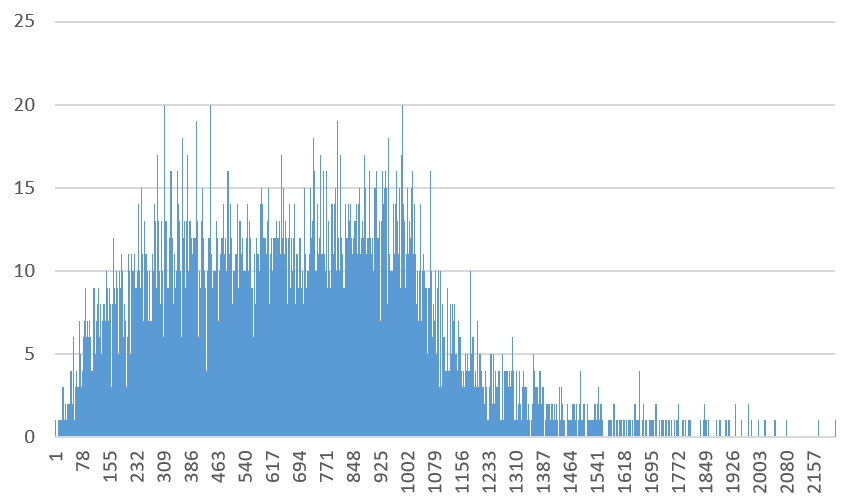
\includegraphics[width=0.7\textwidth]{figures/images/numberGenerator/overlapped.png}\label{fig:overlappedDistExample}
\end{figure}

Figure~\ref{fig:overlappedDistExample} looks completely different from figure~\ref{fig:mixedDistExample}.
No value is generated more than 20 times as opposed to the maximum amount of 350 for the mixed distribution.
In this figure no distribution is clearly visible.

The used distributions were \textasciitilde$U(1,49999)$, \textasciitilde$B(10000,0.1)$, \textasciitilde$Geo(0.001)$, powerlaw distribution with $\beta=-1.25$.
\subsection{RLS Comparison}
The following table lists the results for the RLS for inputs that are chosen from a powerlaw distribution with $\beta=-2.75$.


\makebox[\linewidth]{
\begin{tabular}{lp{3cm}p{6cm}p{6cm}}
\begin{tabular}[h]{cccccccc}
algo type&            RLS&   RLS-R&   RLS-R&   RLS-R&   RLS-N&   RLS-N&   RLS-N\\
algo param&             -&     r=2&     r=3&     r=4&     n=2&     n=3&     n=4\\
avg mut/change&     1.000&   1.181&   1.688&   1.865&   1.997&   3.000&   3.997\\
avg mut/step&       1.000&   1.500&   2.000&   2.500&   2.000&   3.000&   4.000\\
\hline
total avg count&   90,931& 168,311& 236,317& 307,533& 921,030& 921,030& 921,030\\
avg eval count&    90,931& 168,311& 236,317& 307,533&       -&       -&       -\\
max eval count&   156,854& 296,206& 498,474& 595,831&       0&       0&       0\\
min eval count&    64,941& 120,582& 158,304& 212,193&       -&       -&       -\\
\hline
fails&                  0&       0&       0&       0&   1,000&   1,000&   1,000\\
fail ratio&         0.000&   0.000&   0.000&   0.000&   1.000&   1.000&   1.000\\
avg fail dif&           -&       -&       -&       -&      53&      36&     263\\
\end{tabular}
\end{tabular}
}

For these inputs the variants of the RLS perform differently to the binomial input.
The only similarity is the RLS being the worst as the RLS is the only algorithm that did not find an optimal solution for every input.
If the RLS did find an optimal solution in those 5 cases it would instead be the best RLS variant.
The other algorithms are ranked by the probability of flipping only one bit.
This means at first the three RLS-R variants from 2 to 3 to 4 and then the same for the RLS-N variants.
So it does seem like moving mostly one element at once is better for the geometric input in comparison to two elements for the binomial distribution.
In the 5 cases where the RLS did not find an optimal solution it was most likely stuck in a local optimum.

\subsection{(1+1) EA Comparison}
The first table again shows the results for parameter $\beta=-2.75$

\makebox[\linewidth]{
\begin{tabular}{lp{3cm}p{6cm}p{6cm}}
\begin{tabular}[h]{ccccccccc}
algo type&             EA&   EA-SM&   EA-SM&   EA-SM&   EA-SM&   EA-SM&   EA-SM&   EA-SM\\
algo param&             -&     2/n&     3/n&     4/n&     5/n&    10/n&    50/n&   100/n\\
avg mut/change&     1.273&   1.750&   2.334&   2.965&   3.636&   7.288&  45.923&  95.590\\
avg mut/step&       1.000&   2.000&   3.000&   4.000&   5.000&  10.000&  49.998&  100.00\\
\hline
total avg count&  230,328& 297,602& 495,951& 860,736& 921,030& 921,030& 921,030& 921,030\\
avg eval count&   230,328& 297,602& 495,951& 812,983&       -&       -&       -&       -\\
max eval count&   399,393& 625,976& 839,325& 917,029&       -&       -&       -&       -\\
min eval count&   162,400& 193,796& 347,185& 635,812&       -&       -&       -&       -\\
\hline
fails&                  0&       0&       0&      99&     224&     224&     224&     224\\
fail ratio&         0.000&   0.000&   0.000&   0.442&   1.000&   1.000&   1.000&   1.000\\
avg fail dif&           -&       -&       -&       1&      18&     570&   2,488&   3,115\\
\end{tabular}
\end{tabular}
}

For the EA the result is also the inversion of the results for the OneMax equivalent.
The higher the mutation rate the better at least up to $n\le100$.
From mutation rate $p_m\le3/n$ the algorithm reaches the worst case at least once in 1000 runs.
If the algorithm did not manage to find an optimal solution the fitness was always the same.
So there was no run where any algorithm neither found a global nor the local optimum.
\subsection{pmut Comparison}
The first table again shows the results for parameter $\beta=-2.75$

\makebox[\linewidth]{
\scriptsize
\begin{tabular}{lp{3cm}p{6cm}p{6cm}}
\begin{tabular}[h]{cccccccccc}
algo type&           pmut&    pmut&    pmut&    pmut&    pmut&    pmut&    pmut&    pmut&    pmut\\
algo param&         -3.25&   -3.00&   -2.75&   -2.50&   -2.25&   -2.00&   -1.75&   -1.50&   -1.25\\
avg mut/change&     1.289&   1.359&   1.459&   1.591&   1.813&   2.207&   2.760&   3.604&   5.382\\
avg mut/step&       1.731&   1.934&   2.270&   2.907&   4.371&   8.486&  22.299&  70.692& 224.466\\
\hline
total avg count&  145,095& 149,664& 170,912& 181,099& 214,361& 249,102& 301,566& 415,413& 715,219\\
avg eval count&   145,095& 149,664& 170,912& 181,099& 214,361& 249,102& 301,566& 415,413& 683,204\\
max eval count&   217,932& 223,561& 254,330& 246,635& 365,378& 376,768& 431,629& 735,214& 853,181\\
min eval count&   111,061& 119,931& 120,965& 130,174& 161,244& 180,570& 232,166& 311,979& 492,686\\
\hline
fails&                  0&       0&       0&       0&       0&       0&       0&       0&       7\\
fail ratio&         0.000&   0.000&   0.000&   0.000&   0.000&   0.000&   0.000&   0.000&   0.135\\
avg fail dif&           -&       -&       -&       -&       -&       -&       -&       -&       1\\
\end{tabular}
\end{tabular}
}

The ideal value for $\beta$ seems to be around -1.75 as the runtime increases for the two neighbour values.
Even the worst value still manages find an optimal solution within double the time of the best value.
The importance of the parameter is therefore not as important as for other inputs.
\subsection{Comparison of the best variants}
The first table again shows the results for parameter $\beta=-2.75$

\makebox[\linewidth]{
\begin{tabular}{lp{3cm}p{6cm}p{6cm}}
\begin{tabular}[h]{cccc}
algo type&            RLS&    pmut&      EA\\
algo param&             -&   -3.25&       -\\
avg mut/change&     1.000&   1.287&   1.272\\
avg mut/step&       1.000&   1.729&   1.000\\
\hline
total avg count&   91,171& 143,121& 231,082\\
avg eval count&    91,171& 143,121& 231,082\\
max eval count&   153,143& 227,737& 446,942\\
min eval count&    65,783&  93,602& 165,818\\
\hline
fails&                  0&       0&       0\\
fail ratio&         0.000&   0.000&   0.000\\
avg fail dif&           -&       -&       -\\
\end{tabular}
\end{tabular}
}

The results for this experiment are as expected.
All three algorithms find the optimal value within the time limit.
The RLS performs better than the (1+1) EA because it does only single bit flips.
The $pmut_{-3.25}$ perform better than the standard (1+1) EA although flipping more bits on average.
This is most likely cause by the few steps where $pmut$ flips many bits which increase the average.
But $pmut$ most likely chooses to flip only one bit more often as the (1+1) EA.

TODO insert comparison with multiple values of n.
\section{Carsten Witts worst case input}
This input is similar to the mixed input from the last subsection.
For this distribution the values are not chosen uniform random from one of the base distributions, but instead a value from every distribution is chosen and added together.
Hence the name overlapped distribution.
For this input the step limit was increased to $100\cdot n \ln n$.
The comparison with the step limit $10\cdot n \ln(n)$ is contained in the last subsubsection which compares the best variants.

\begin{figure}[h]
      \caption{Distribution of an overlapped input with \textasciitilde$U(1,999)$, \textasciitilde$B(1000,0.1)$, \textasciitilde$Geo(0.01)$, powerlaw dist with $\beta=-1.25$}
      \centering
      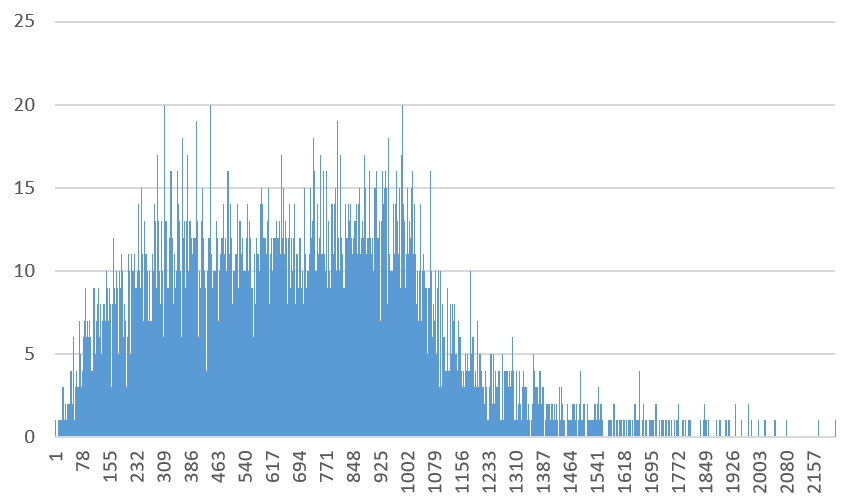
\includegraphics[width=0.7\textwidth]{figures/images/numberGenerator/overlapped.png}\label{fig:overlappedDistExample}
\end{figure}

Figure~\ref{fig:overlappedDistExample} looks completely different from figure~\ref{fig:mixedDistExample}.
No value is generated more than 20 times as opposed to the maximum amount of 350 for the mixed distribution.
In this figure no distribution is clearly visible.

The used distributions were \textasciitilde$U(1,49999)$, \textasciitilde$B(10000,0.1)$, \textasciitilde$Geo(0.001)$, powerlaw distribution with $\beta=-1.25$.
\subsection{RLS Comparison}
The following table lists the results for the RLS for inputs that are chosen from a powerlaw distribution with $\beta=-2.75$.


\makebox[\linewidth]{
\begin{tabular}{lp{3cm}p{6cm}p{6cm}}
\begin{tabular}[h]{cccccccc}
algo type&         RLS-N&  RLS-R&  RLS-R&  RLS-R&  RLS-N&    RLS&  RLS-N\\
algo param&          n=3&    r=4&    r=3&    r=2&    n=4&      -&    n=2\\
avg mut/change&    3.000&  2.379&  1.985&  1.327&  3.997&  1.000&  1.998\\
avg mut/step&      3.000&  2.500&  2.000&  1.500&  4.000&  1.000&  2.000\\
\hline
total avg count&   1,436&  1,641&  1,905&  2,856&  4,420&  6,507&  6,693\\
avg eval count&    1,436&  1,641&  1,905&  2,856&  4,420&  3,755&  6,693\\
max eval count&   12,521& 15,338& 22,394& 26,297& 42,702& 31,837& 74,281\\
min eval count&        0&      0&      0&      0&      0&      0&      0\\
\hline
fails&                 0&      0&      0&      0&      0&      3&      0\\
fail ratio&        0.000&  0.000&  0.000&  0.000&  0.000&  0.003&  0.000\\
avg fail dif&          -&      -&      -&      -&      -&  4,249&      -\\
\end{tabular}
\end{tabular}
}

For these inputs the variants of the RLS perform differently to the binomial input.
The only similarity is the RLS being the worst as the RLS is the only algorithm that did not find an optimal solution for every input.
If the RLS did find an optimal solution in those 5 cases it would instead be the best RLS variant.
The other algorithms are ranked by the probability of flipping only one bit.
This means at first the three RLS-R variants from 2 to 3 to 4 and then the same for the RLS-N variants.
So it does seem like moving mostly one element at once is better for the geometric input in comparison to two elements for the binomial distribution.
In the 5 cases where the RLS did not find an optimal solution it was most likely stuck in a local optimum.

\subsection{(1+1) EA Comparison}
The first table again shows the results for parameter $\beta=-2.75$

\makebox[\linewidth]{
\begin{tabular}{lp{3cm}p{6cm}p{6cm}}
\begin{tabular}[h]{ccccccccc}
algo type&         EA-SM&  EA-SM&  EA-SM&  EA-SM&  EA-SM&  EA-SM&  EA-SM&     EA\\
algo param&        100/n&   50/n&   10/n&    5/n&    4/n&    3/n&    2/n&      -\\
avg mut/change&   99.982& 49.983& 10.028&  5.085&  4.112&  3.150&  2.244&  1.470\\
avg mut/step&     99.980& 49.975& 10.002&  5.001&  4.001&  3.000&  2.001&  1.000\\
\hline
total avg count&      73&     97&    397&    839&    966&  1,391&  1,827&  3,732\\
avg eval count&       73&     97&    397&    839&    966&  1,391&  1,827&  3,732\\
max eval count&      488&    736&  5,075&  8,348&  9,734& 14,546& 22,186& 44,370\\
min eval count&        0&      0&      0&      0&      0&      0&      0&      0\\
\hline
fails&                 0&      0&      0&      0&      0&      0&      0&      0\\
fail ratio&        0.000&  0.000&  0.000&  0.000&  0.000&  0.000&  0.000&  0.000\\
avg fail dif&          -&      -&      -&      -&      -&      -&      -&      -\\
\end{tabular}
\end{tabular}
}

For the EA the result is also the inversion of the results for the OneMax equivalent.
The higher the mutation rate the better at least up to $n\le100$.
From mutation rate $p_m\le3/n$ the algorithm reaches the worst case at least once in 1000 runs.
If the algorithm did not manage to find an optimal solution the fitness was always the same.
So there was no run where any algorithm neither found a global nor the local optimum.
\subsection{pmut Comparison}
The first table again shows the results for parameter $\beta=-2.75$

\makebox[\linewidth]{
\scriptsize
\begin{tabular}{lp{3cm}p{6cm}p{6cm}}
\begin{tabular}[h]{cccccccccc}
algo type&           pmut&    pmut&    pmut&    pmut&    pmut&    pmut&    pmut&    pmut&    pmut\\
algo param&         -1.25&   -1.50&   -1.75&   -2.00&   -2.25&   -2.50&   -2.75&   -3.00&   -3.25\\
avg mut/change&   197.675&  69.384&  23.211&   8.999&   4.259&   2.819&   2.133&   1.802&   1.598\\
avg mut/step&     226.848&  69.933&  22.429&   8.747&   4.313&   2.911&   2.268&   1.934&   1.725\\
\hline
total avg count&       41&      85&     222&     536&     922&   1,368&   1,723&   2,080&   2,339\\
avg eval count&        41&      85&     222&     536&     922&   1,368&   1,723&   2,080&   2,339\\
max eval count&       226&     682&   2,033&   4,760&   9,749&  16,271&  18,953&  18,794&  25,383\\
min eval count&         0&       0&       0&       0&       0&       0&       0&       0&       0\\
\hline
fails&                  0&       0&       0&       0&       0&       0&       0&       0&       0\\
fail ratio&         0.000&   0.000&   0.000&   0.000&   0.000&   0.000&   0.000&   0.000&   0.000\\
avg fail dif&           -&       -&       -&       -&       -&       -&       -&       -&       -\\
\end{tabular}
\end{tabular}
}

The ideal value for $\beta$ seems to be around -1.75 as the runtime increases for the two neighbour values.
Even the worst value still manages find an optimal solution within double the time of the best value.
The importance of the parameter is therefore not as important as for other inputs.
\subsection{Comparison of the best variants}
The first table again shows the results for parameter $\beta=-2.75$

\makebox[\linewidth]{
\begin{tabular}{lp{3cm}p{6cm}p{6cm}}
\begin{tabular}[h]{cccc}
algo type&           pmut&   EA-SM&   RLS-N\\
algo param&         -1.25&   100/n&     k=3\\
avg mut/change&   208.477&  99.891&   3.000\\
avg mut/step&     228.998& 100.014&   3.000\\
\hline
total avg count&       42&      68&   1,216\\
avg eval count&        42&      68&   1,216\\
max eval count&       231&     466&  13,896\\
min eval count&         0&       0&       0\\
\hline
fails&                  0&       0&       0\\
fail ratio&         0.000&   0.000&   0.000\\
avg fail dif&           -&       -&       -\\
\end{tabular}
\end{tabular}
}

The results for this experiment are as expected.
All three algorithms find the optimal value within the time limit.
The RLS performs better than the (1+1) EA because it does only single bit flips.
The $pmut_{-3.25}$ perform better than the standard (1+1) EA although flipping more bits on average.
This is most likely cause by the few steps where $pmut$ flips many bits which increase the average.
But $pmut$ most likely chooses to flip only one bit more often as the (1+1) EA.

TODO insert comparison with multiple values of n.
\section{Multiple distributions overlapped}
This input is similar to the mixed input from the last subsection.
For this distribution the values are not chosen uniform random from one of the base distributions, but instead a value from every distribution is chosen and added together.
Hence the name overlapped distribution.
For this input the step limit was increased to $100\cdot n \ln n$.
The comparison with the step limit $10\cdot n \ln(n)$ is contained in the last subsubsection which compares the best variants.

\begin{figure}[h]
      \caption{Distribution of an overlapped input with \textasciitilde$U(1,999)$, \textasciitilde$B(1000,0.1)$, \textasciitilde$Geo(0.01)$, powerlaw dist with $\beta=-1.25$}
      \centering
      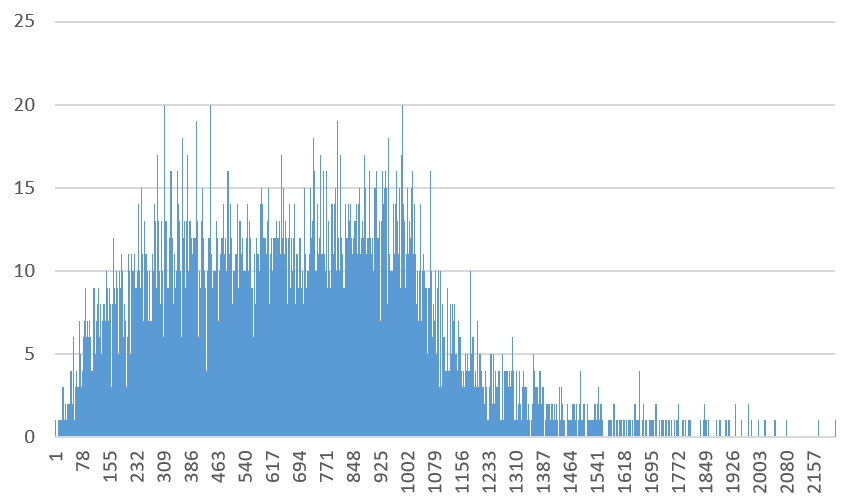
\includegraphics[width=0.7\textwidth]{figures/images/numberGenerator/overlapped.png}\label{fig:overlappedDistExample}
\end{figure}

Figure~\ref{fig:overlappedDistExample} looks completely different from figure~\ref{fig:mixedDistExample}.
No value is generated more than 20 times as opposed to the maximum amount of 350 for the mixed distribution.
In this figure no distribution is clearly visible.

The used distributions were \textasciitilde$U(1,49999)$, \textasciitilde$B(10000,0.1)$, \textasciitilde$Geo(0.001)$, powerlaw distribution with $\beta=-1.25$.
\subsection{RLS Comparison}
The following table lists the results for the RLS for inputs that are chosen from a powerlaw distribution with $\beta=-2.75$.


\makebox[\linewidth]{
\begin{tabular}{lp{3cm}p{6cm}p{6cm}}
\begin{tabular}[h]{cccccccc}
algo type&           RLS-R&    RLS-R&    RLS-R&    RLS-N&    RLS-N&      RLS&    RLS-N\\
algo param&            r=4&      r=3&      r=2&      n=3&      n=2&        -&      n=4\\
avg mut/change&      2.413&    1.951&    1.478&    2.000&    1.000&    1.000&    3.000\\
avg mut/step&        2.503&    2.000&    1.500&    2.000&    1.000&    1.000&    3.000\\
\hline
total avg count&       539&      546&      608&      612&      729&      733&      930\\
avg eval count&        539&      546&      608&      612&      729&      733&      930\\
max eval count&      1,579&    1,661&    1,883&    2,629&    2,623&    2,371&    4,591\\
min eval count&         15&        8&       42&       53&       80&       59&       73\\
\hline
fails&                   0&        0&        0&        0&        0&        0&        0\\
fail ratio&          0.000&    0.000&    0.000&    0.000&    0.000&    0.000&    0.000\\
avg fail dif&            -&        -&        -&        -&        -&        -&        -\\
\end{tabular}
\end{tabular}
}

For these inputs the variants of the RLS perform differently to the binomial input.
The only similarity is the RLS being the worst as the RLS is the only algorithm that did not find an optimal solution for every input.
If the RLS did find an optimal solution in those 5 cases it would instead be the best RLS variant.
The other algorithms are ranked by the probability of flipping only one bit.
This means at first the three RLS-R variants from 2 to 3 to 4 and then the same for the RLS-N variants.
So it does seem like moving mostly one element at once is better for the geometric input in comparison to two elements for the binomial distribution.
In the 5 cases where the RLS did not find an optimal solution it was most likely stuck in a local optimum.

\subsection{(1+1) EA Comparison}
The first table again shows the results for parameter $\beta=-2.75$

\makebox[\linewidth]{
\begin{tabular}{lp{3cm}p{6cm}p{6cm}}
\begin{tabular}[h]{ccccccc}
algo type&             EA-SM&      EA-SM&      EA-SM&         EA&      EA-SM&      EA-SM\\
algo param&              3/n&        2/n&        4/n&          -&        5/n&       10/n\\
avg mut/change&        3.009&      2.230&      3.863&      1.545&      4.762&      9.548\\
avg mut/step&          3.000&      2.000&      3.998&      0.999&      4.998&     10.000\\
\hline
total avg count&         599&        617&        701&        942&        968&     11,682\\
avg eval count&          599&        617&        701&        942&        968&     11,682\\
max eval count&        1,927&      1,769&      2,016&      3,284&      3,537&     63,180\\
min eval count&           56&         65&         85&         91&         51&        112\\
\hline
fails&                     0&          0&          0&          0&          0&          0\\
fail ratio&            0.000&      0.000&      0.000&      0.000&      0.000&      0.000\\
avg fail dif&              -&          -&          -&          -&          -&          -\\
\end{tabular}
\end{tabular}
}

For the EA the result is also the inversion of the results for the OneMax equivalent.
The higher the mutation rate the better at least up to $n\le100$.
From mutation rate $p_m\le3/n$ the algorithm reaches the worst case at least once in 1000 runs.
If the algorithm did not manage to find an optimal solution the fitness was always the same.
So there was no run where any algorithm neither found a global nor the local optimum.
\subsection{pmut Comparison}
The first table again shows the results for parameter $\beta=-2.75$

\makebox[\linewidth]{
\scriptsize
\begin{tabular}{lp{3cm}p{6cm}p{6cm}}
\begin{tabular}[h]{cccccccccc}
algo type&             pmut&      pmut&      pmut&      pmut&      pmut&      pmut&      pmut&      pmut&      pmut\\
algo param&           -1.75&     -2.00&     -2.25&     -1.50&     -2.50&     -2.75&     -3.00&     -3.25&     -1.25\\
avg mut/change&      29.356&     9.267&     3.910&   123.650&     2.761&     2.150&     1.855&     1.673&   399.522\\
avg mut/step&        40.906&    10.981&     4.619&   226.724&     2.950&     2.256&     1.935&     1.729&  1192.167\\
\hline
total avg count&        454&       479&       501&       504&       515&       541&       555&       572&       722\\
avg eval count&         454&       479&       501&       504&       515&       541&       555&       572&       722\\
max eval count&       1,404&     1,423&     1,437&     1,606&     1,988&     1,434&     1,444&     1,800&     2,223\\
min eval count&          38&        19&        45&        47&        18&        18&        58&        27&        48\\
\hline
fails&                    0&         0&         0&         0&         0&         0&         0&         0&         0\\
fail ratio&           0.000&     0.000&     0.000&     0.000&     0.000&     0.000&     0.000&     0.000&     0.000\\
avg fail dif&             -&         -&         -&         -&         -&         -&         -&         -&         -\\
\end{tabular}
\end{tabular}
}

The ideal value for $\beta$ seems to be around -1.75 as the runtime increases for the two neighbour values.
Even the worst value still manages find an optimal solution within double the time of the best value.
The importance of the parameter is therefore not as important as for other inputs.
\subsection{Comparison of the best variants}
The first table again shows the results for parameter $\beta=-2.75$

\makebox[\linewidth]{
\begin{tabular}{lp{3cm}p{6cm}p{6cm}}
\begin{tabular}[h]{cccc}
algo type&            pmut&    RLS-R&    EA-SM\\
algo param&          -1.75&      r=4&      3/n\\
avg mut/change&     30.999&    2.415&    3.015\\
avg mut/step&       42.499&    2.501&    3.002\\
\hline
total avg count&       463&      543&      586\\
avg eval count&        463&      543&      586\\
max eval count&      1,330&    1,613&    1,389\\
min eval count&         61&       50&       99\\
\hline
fails&                   0&        0&        0\\
fail ratio&          0.000&    0.000&    0.000\\
avg fail dif&            -&        -&        -\\
\end{tabular}
\end{tabular}
}

The results for this experiment are as expected.
All three algorithms find the optimal value within the time limit.
The RLS performs better than the (1+1) EA because it does only single bit flips.
The $pmut_{-3.25}$ perform better than the standard (1+1) EA although flipping more bits on average.
This is most likely cause by the few steps where $pmut$ flips many bits which increase the average.
But $pmut$ most likely chooses to flip only one bit more often as the (1+1) EA.

TODO insert comparison with multiple values of n.
\section{Multiple distributions mixed}
This input is similar to the mixed input from the last subsection.
For this distribution the values are not chosen uniform random from one of the base distributions, but instead a value from every distribution is chosen and added together.
Hence the name overlapped distribution.
For this input the step limit was increased to $100\cdot n \ln n$.
The comparison with the step limit $10\cdot n \ln(n)$ is contained in the last subsubsection which compares the best variants.

\begin{figure}[h]
      \caption{Distribution of an overlapped input with \textasciitilde$U(1,999)$, \textasciitilde$B(1000,0.1)$, \textasciitilde$Geo(0.01)$, powerlaw dist with $\beta=-1.25$}
      \centering
      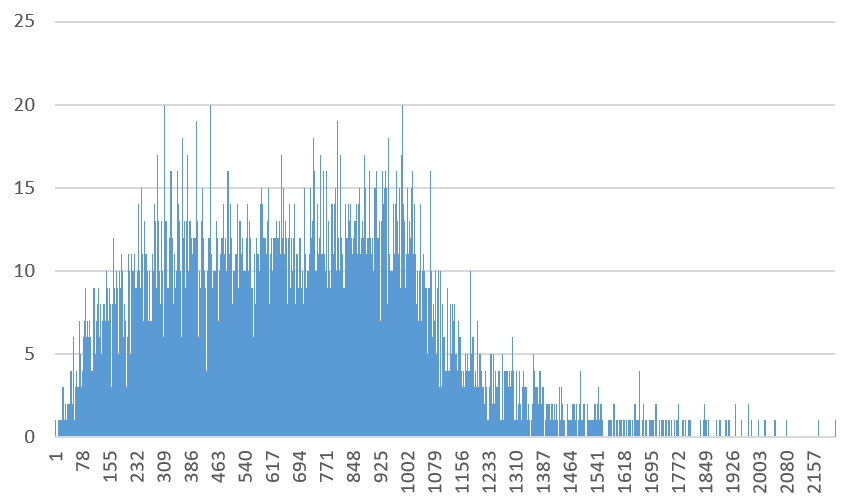
\includegraphics[width=0.7\textwidth]{figures/images/numberGenerator/overlapped.png}\label{fig:overlappedDistExample}
\end{figure}

Figure~\ref{fig:overlappedDistExample} looks completely different from figure~\ref{fig:mixedDistExample}.
No value is generated more than 20 times as opposed to the maximum amount of 350 for the mixed distribution.
In this figure no distribution is clearly visible.

The used distributions were \textasciitilde$U(1,49999)$, \textasciitilde$B(10000,0.1)$, \textasciitilde$Geo(0.001)$, powerlaw distribution with $\beta=-1.25$.
\subsection{RLS Comparison}
The following table lists the results for the RLS for inputs that are chosen from a powerlaw distribution with $\beta=-2.75$.


\makebox[\linewidth]{
\begin{tabular}{lp{3cm}p{6cm}p{6cm}}
\begin{tabular}[h]{cccccccc}
algo type&               RLS-N&        RLS-R&        RLS-R&        RLS-R&        RLS-N&        RLS-N&          RLS\\
algo param&                n=3&          r=4&          r=3&          r=2&          n=4&          n=2&            -\\
avg mut/change&          2.000&        2.556&        2.059&        1.593&        3.000&          NaN&          NaN\\
avg mut/step&            2.000&        2.501&        2.000&        1.500&        3.000&          NaN&          NaN\\
\hline
total avg count&       125,951&      249,157&      265,643&      268,552&      307,558&    9,210,300&    9,210,300\\
avg eval count&        125,951&      249,157&      265,643&      268,552&      307,558&            -&            -\\
max eval count&        862,008&    1,939,594&    2,389,907&    2,012,463&    2,203,167&            -&            -\\
min eval count&            155&          276&          331&          267&          156&            -&            -\\
\hline
fails&                       0&            0&            0&            0&            0&        1,000&        1,000\\
fail ratio&              0.000&        0.000&        0.000&        0.000&        0.000&        1.000&        1.000\\
avg fail dif&                -&            -&            -&            -&            -&          778&          785\\
\end{tabular}
\end{tabular}
}

For these inputs the variants of the RLS perform differently to the binomial input.
The only similarity is the RLS being the worst as the RLS is the only algorithm that did not find an optimal solution for every input.
If the RLS did find an optimal solution in those 5 cases it would instead be the best RLS variant.
The other algorithms are ranked by the probability of flipping only one bit.
This means at first the three RLS-R variants from 2 to 3 to 4 and then the same for the RLS-N variants.
So it does seem like moving mostly one element at once is better for the geometric input in comparison to two elements for the binomial distribution.
In the 5 cases where the RLS did not find an optimal solution it was most likely stuck in a local optimum.

\subsection{(1+1) EA Comparison}
The first table again shows the results for parameter $\beta=-2.75$

\makebox[\linewidth]{
\begin{tabular}{lp{3cm}p{6cm}p{6cm}}
\begin{tabular}[h]{ccccccc}
algo type&               EA-SM&        EA-SM&        EA-SM&        EA-SM&        EA-SM&           EA\\
algo param&                4/n&          3/n&          5/n&          2/n&         10/n&            -\\
avg mut/change&          3.981&        3.153&        4.887&        2.359&        9.759&        1.701\\
avg mut/step&            4.000&        3.000&        5.000&        2.000&       10.000&        1.000\\
\hline
total avg count&       244,704&      253,722&      268,529&      304,147&      346,669&      577,955\\
avg eval count&        244,704&      253,722&      268,529&      304,147&      346,669&      577,955\\
max eval count&      2,209,416&    2,340,925&    2,589,980&    2,416,509&    2,474,967&    3,776,445\\
min eval count&            269&          405&           24&          177&          236&           89\\
\hline
fails&                       0&            0&            0&            0&            0&            0\\
fail ratio&              0.000&        0.000&        0.000&        0.000&        0.000&        0.000\\
avg fail dif&                -&            -&            -&            -&            -&            -\\
\end{tabular}
\end{tabular}
}

For the EA the result is also the inversion of the results for the OneMax equivalent.
The higher the mutation rate the better at least up to $n\le100$.
From mutation rate $p_m\le3/n$ the algorithm reaches the worst case at least once in 1000 runs.
If the algorithm did not manage to find an optimal solution the fitness was always the same.
So there was no run where any algorithm neither found a global nor the local optimum.
\subsection{pmut Comparison}
The first table again shows the results for parameter $\beta=-2.75$

\makebox[\linewidth]{
\scriptsize
\begin{tabular}{lp{3cm}p{6cm}p{6cm}}
\begin{tabular}[h]{cccccccccc}
algo type&                pmut&         pmut&         pmut&         pmut&         pmut&         pmut&         pmut&         pmut&         pmut\\
algo param&              -2.00&        -2.25&        -1.75&        -2.50&        -2.75&        -1.50&        -3.00&        -3.25&        -1.25\\
avg mut/change&          6.738&        4.132&       14.905&        2.817&        2.298&       37.736&        2.008&        1.832&       96.985\\
avg mut/step&            8.485&        4.364&       22.232&        2.906&        2.271&       70.714&        1.934&        1.729&      224.557\\
\hline
total avg count&       292,521&      292,763&      304,924&      307,403&      322,391&      337,925&      356,686&      377,068&      419,335\\
avg eval count&        292,521&      292,763&      304,924&      307,403&      322,391&      337,925&      356,686&      377,068&      419,335\\
max eval count&      3,811,952&    1,930,058&    2,875,275&    2,364,678&    2,233,600&    4,824,371&    2,832,218&    3,395,371&    3,133,351\\
min eval count&            535&          251&          202&          105&          124&          560&          104&           52&          841\\
\hline
fails&                       0&            0&            0&            0&            0&            0&            0&            0&            0\\
fail ratio&              0.000&        0.000&        0.000&        0.000&        0.000&        0.000&        0.000&        0.000&        0.000\\
avg fail dif&                -&            -&            -&            -&            -&            -&            -&            -&            -\\
\end{tabular}
\end{tabular}
}

The ideal value for $\beta$ seems to be around -1.75 as the runtime increases for the two neighbour values.
Even the worst value still manages find an optimal solution within double the time of the best value.
The importance of the parameter is therefore not as important as for other inputs.
\subsection{Comparison of the best variants}
The first table again shows the results for parameter $\beta=-2.75$

\makebox[\linewidth]{
\begin{tabular}{lp{3cm}p{6cm}p{6cm}}
\begin{tabular}[h]{cccc}
algo type&               RLS-N&        EA-SM&         pmut\\
algo param&                n=3&          4/n&        -2.00\\
avg mut/change&          2.000&        3.996&        7.729\\
avg mut/step&            2.000&        4.000&        8.477\\
\hline
total avg count&       129,281&      267,444&      311,741\\
avg eval count&        129,281&      267,444&      311,741\\
max eval count&      1,276,682&    1,958,436&    2,465,518\\
min eval count&             62&          385&          245\\
\hline
fails&                       0&            0&            0\\
fail ratio&              0.000&        0.000&        0.000\\
avg fail dif&                -&            -&            -\\
\end{tabular}
\end{tabular}
}

The results for this experiment are as expected.
All three algorithms find the optimal value within the time limit.
The RLS performs better than the (1+1) EA because it does only single bit flips.
The $pmut_{-3.25}$ perform better than the standard (1+1) EA although flipping more bits on average.
This is most likely cause by the few steps where $pmut$ flips many bits which increase the average.
But $pmut$ most likely chooses to flip only one bit more often as the (1+1) EA.

TODO insert comparison with multiple values of n.
\section{Multiple distributions mixed \& overlapped}
This input is similar to the mixed input from the last subsection.
For this distribution the values are not chosen uniform random from one of the base distributions, but instead a value from every distribution is chosen and added together.
Hence the name overlapped distribution.
For this input the step limit was increased to $100\cdot n \ln n$.
The comparison with the step limit $10\cdot n \ln(n)$ is contained in the last subsubsection which compares the best variants.

\begin{figure}[h]
      \caption{Distribution of an overlapped input with \textasciitilde$U(1,999)$, \textasciitilde$B(1000,0.1)$, \textasciitilde$Geo(0.01)$, powerlaw dist with $\beta=-1.25$}
      \centering
      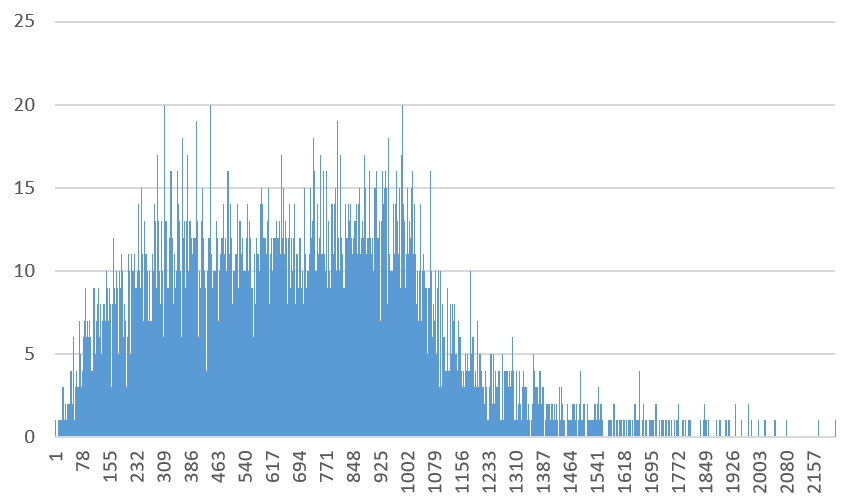
\includegraphics[width=0.7\textwidth]{figures/images/numberGenerator/overlapped.png}\label{fig:overlappedDistExample}
\end{figure}

Figure~\ref{fig:overlappedDistExample} looks completely different from figure~\ref{fig:mixedDistExample}.
No value is generated more than 20 times as opposed to the maximum amount of 350 for the mixed distribution.
In this figure no distribution is clearly visible.

The used distributions were \textasciitilde$U(1,49999)$, \textasciitilde$B(10000,0.1)$, \textasciitilde$Geo(0.001)$, powerlaw distribution with $\beta=-1.25$.
\subsection{RLS Comparison}
The following table lists the results for the RLS for inputs that are chosen from a powerlaw distribution with $\beta=-2.75$.


\makebox[\linewidth]{
\begin{tabular}{lp{3cm}p{6cm}p{6cm}}
\begin{tabular}[h]{cccccccc}
algo type&            RLS-N&     RLS-R&     RLS-R&     RLS-R&       RLS&     RLS-N&     RLS-N\\
algo param&             n=3&       r=3&       r=2&       r=4&         -&       n=2&       n=4\\
avg mut/change&       2.000&     1.903&     1.468&     2.321&     1.000&     1.000&     3.000\\
avg mut/step&         2.000&     2.001&     1.500&     2.500&     1.000&     1.000&     3.000\\
\hline
total avg count&      1,193&     1,326&     1,348&     1,406&     1,776&     1,780&     1,850\\
avg eval count&       1,193&     1,326&     1,348&     1,406&     1,776&     1,780&     1,850\\
max eval count&       3,692&     3,666&     3,490&     3,833&     4,568&     4,700&     5,159\\
min eval count&          44&        65&        94&        33&       109&        55&       102\\
\hline
fails&                    0&         0&         0&         0&         0&         0&         0\\
fail ratio&           0.000&     0.000&     0.000&     0.000&     0.000&     0.000&     0.000\\
avg fail dif&             -&         -&         -&         -&         -&         -&         -\\
\end{tabular}
\end{tabular}
}

For these inputs the variants of the RLS perform differently to the binomial input.
The only similarity is the RLS being the worst as the RLS is the only algorithm that did not find an optimal solution for every input.
If the RLS did find an optimal solution in those 5 cases it would instead be the best RLS variant.
The other algorithms are ranked by the probability of flipping only one bit.
This means at first the three RLS-R variants from 2 to 3 to 4 and then the same for the RLS-N variants.
So it does seem like moving mostly one element at once is better for the geometric input in comparison to two elements for the binomial distribution.
In the 5 cases where the RLS did not find an optimal solution it was most likely stuck in a local optimum.

\subsection{(1+1) EA Comparison}
The first table again shows the results for parameter $\beta=-2.75$

\makebox[\linewidth]{
\begin{tabular}{lp{3cm}p{6cm}p{6cm}}
\begin{tabular}[h]{ccccccc}
algo type&             EA-SM&      EA-SM&      EA-SM&         EA&      EA-SM&      EA-SM\\
algo param&              3/n&        2/n&        4/n&          -&        5/n&       10/n\\
avg mut/change&        2.883&      2.146&      3.698&      1.514&      4.583&      9.553\\
avg mut/step&          3.000&      2.002&      4.000&      1.001&      5.001&     10.000\\
\hline
total avg count&       1,577&      1,648&      1,938&      2,224&      2,579&     22,183\\
avg eval count&        1,577&      1,648&      1,938&      2,224&      2,579&     22,183\\
max eval count&        4,466&      4,510&      5,481&      6,566&      8,345&     93,948\\
min eval count&           66&        169&        159&        232&        179&        225\\
\hline
fails&                     0&          0&          0&          0&          0&          0\\
fail ratio&            0.000&      0.000&      0.000&      0.000&      0.000&      0.000\\
avg fail dif&              -&          -&          -&          -&          -&          -\\
\end{tabular}
\end{tabular}
}

For the EA the result is also the inversion of the results for the OneMax equivalent.
The higher the mutation rate the better at least up to $n\le100$.
From mutation rate $p_m\le3/n$ the algorithm reaches the worst case at least once in 1000 runs.
If the algorithm did not manage to find an optimal solution the fitness was always the same.
So there was no run where any algorithm neither found a global nor the local optimum.
\subsection{pmut Comparison}
The first table again shows the results for parameter $\beta=-2.75$

\makebox[\linewidth]{
\scriptsize
\begin{tabular}{lp{3cm}p{6cm}p{6cm}}
\begin{tabular}[h]{cccccccccc}
algo type&             pmut&      pmut&      pmut&      pmut&      pmut&      pmut&      pmut&      pmut&      pmut\\
algo param&           -2.50&     -2.25&     -2.75&     -2.00&     -3.25&     -3.00&     -1.75&     -1.50&     -1.25\\
avg mut/change&       2.500&     3.777&     2.053&     7.773&     1.622&     1.785&    22.640&    97.028&   310.342\\
avg mut/step&         2.914&     4.680&     2.271&    10.908&     1.733&     1.928&    41.606&   222.441&  1196.549\\
\hline
total avg count&      1,368&     1,395&     1,418&     1,422&     1,423&     1,428&     1,554&     1,797&     2,493\\
avg eval count&       1,368&     1,395&     1,418&     1,422&     1,423&     1,428&     1,554&     1,797&     2,493\\
max eval count&       4,195&     4,235&     4,599&     4,348&     4,609&     4,040&     4,775&     5,609&     8,303\\
min eval count&         133&        90&        49&        23&        95&        99&        94&       134&        87\\
\hline
fails&                    0&         0&         0&         0&         0&         0&         0&         0&         0\\
fail ratio&           0.000&     0.000&     0.000&     0.000&     0.000&     0.000&     0.000&     0.000&     0.000\\
avg fail dif&             -&         -&         -&         -&         -&         -&         -&         -&         -\\
\end{tabular}
\end{tabular}
}

The ideal value for $\beta$ seems to be around -1.75 as the runtime increases for the two neighbour values.
Even the worst value still manages find an optimal solution within double the time of the best value.
The importance of the parameter is therefore not as important as for other inputs.
\subsection{Comparison of the best variants}
The first table again shows the results for parameter $\beta=-2.75$

\makebox[\linewidth]{
\begin{tabular}{lp{3cm}p{6cm}p{6cm}}
\begin{tabular}[h]{cccc}
algo type&            RLS-N&      pmut&     EA-SM\\
algo param&             n=3&     -2.50&       3/n\\
avg mut/change&       2.000&     2.875&     2.882\\
avg mut/step&         2.000&     2.972&     3.000\\
\hline
total avg count&      1,225&     1,424&     1,579\\
avg eval count&       1,225&     1,424&     1,579\\
max eval count&       3,347&     3,791&     4,611\\
min eval count&          50&       139&       103\\
\hline
fails&                    0&         0&         0\\
fail ratio&           0.000&     0.000&     0.000\\
avg fail dif&             -&         -&         -\\
\end{tabular}
\end{tabular}
}

The results for this experiment are as expected.
All three algorithms find the optimal value within the time limit.
The RLS performs better than the (1+1) EA because it does only single bit flips.
The $pmut_{-3.25}$ perform better than the standard (1+1) EA although flipping more bits on average.
This is most likely cause by the few steps where $pmut$ flips many bits which increase the average.
But $pmut$ most likely chooses to flip only one bit more often as the (1+1) EA.

TODO insert comparison with multiple values of n.
